\begin{figure*}[htbp]
    \centering
    
    % --- STOLPEC (a) ---
    \begin{subfigure}[b]{0.24\textwidth}
        \centering
        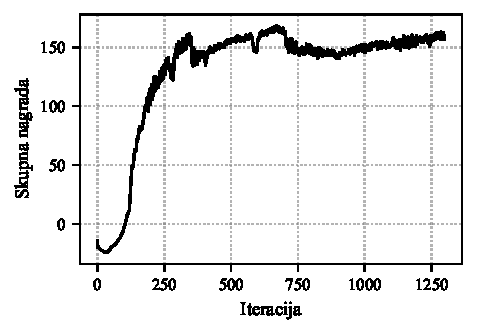
\includegraphics[width=\textwidth]{Images/Episode_reward.pdf}
        \caption{}
        \label{Nagrada}
    \end{subfigure}
    \hfill % Avtomatski vodoravni razmak med stolpci
  % --- STOLPEC (b) ---
    \begin{subfigure}[b]{0.24\textwidth}
        \centering
        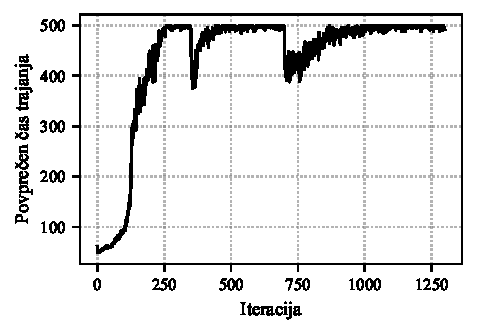
\includegraphics[width=\textwidth]{Images/Episode_length.pdf}
        \caption{}
        \label{Dolžina epizode}
    \end{subfigure}
    \hfill % Avtomatski vodoravni razmak med stolpci
  % --- STOLPEC (d) ---
    \begin{subfigure}[b]{0.24\textwidth}
        \centering
        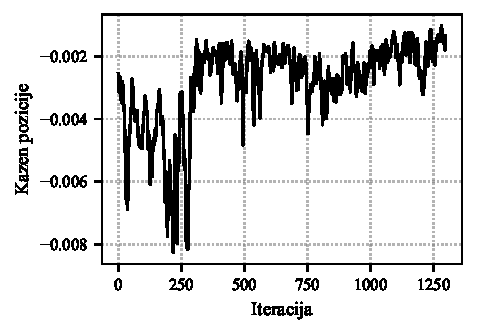
\includegraphics[width=\textwidth]{Images/Position_reward.pdf}
        \caption{}
        \label{Kazen pozicije}
    \end{subfigure}
    \hfill % Avtomatski vodoravni razmak med stolpci
    % --- STOLPEC (c) ---
    \begin{subfigure}[b]{0.24\textwidth}
        \centering
        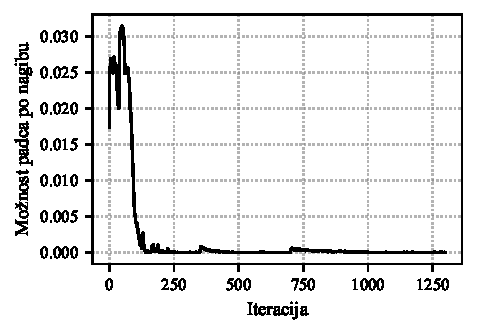
\includegraphics[width=\textwidth]{Images/Roll_fall_rate.pdf}
        \caption{}
        \label{Padec nagiba}
    \end{subfigure}
    \hfill % Avtomatski vodoravni razmak med stolpci
      % --- STOLPEC (c) ---
    \begin{subfigure}[b]{0.24\textwidth}
        \centering
        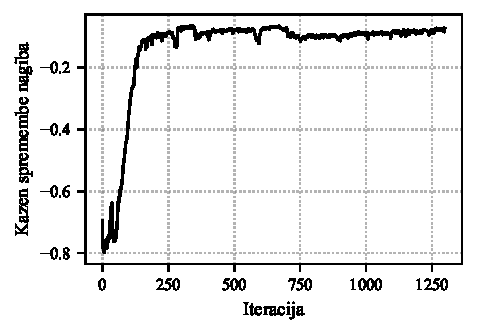
\includegraphics[width=\textwidth]{Images/Rollrate_penalty.pdf}
        \caption{}
        \label{Hitrost nagiba}
    \end{subfigure}
    \hfill % Avtomatski vodoravni razmak med stolpci
    % --- STOLPEC (c) ---
    \begin{subfigure}[b]{0.24\textwidth}
        \centering
        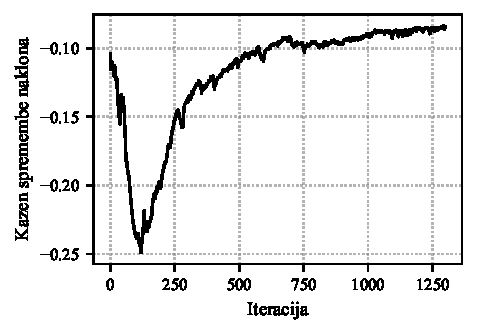
\includegraphics[width=\textwidth]{Images/Pitchrate_penalty.pdf}
        \caption{}
        \label{Hitrost naklona}
    \end{subfigure}
    \hfill % Avtomatski vodoravni razmak med stolpci
      % --- STOLPEC (c) ---
    \begin{subfigure}[b]{0.24\textwidth}
        \centering
        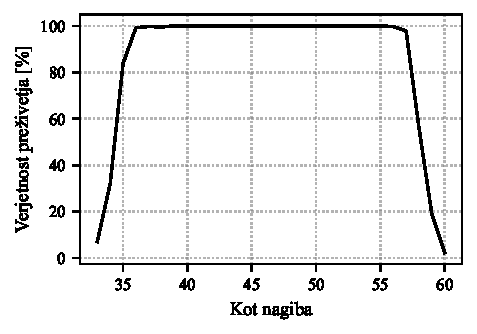
\includegraphics[width=\textwidth]{Images/survival_rate.pdf}
        \caption{}
        \label{Verjetnost preživetja}
    \end{subfigure}
    \hfill % Avtomatski vodoravni razmak med stolpci

    \caption{(a) Nagrada na epizodo, (b) Povprečen čas trajanja epizode, (c) Kazen pozicije na epizodo, (d) Možnost padca po nagiba v vsakem koraku, (e) Kazen spremembe kota nagiba, (f) Kazen spremembe kota naklona, (g) Verjetnost preživetja glede na začetni kot nagiba.}
    \label{fig:glavna_slika_6}
\end{figure*} 

\section{Eksperimentalni rezultati}
Posluževanje večfaznega učenja je očitno vidno predvsem v grafih \ref{Nagrada}, \ref{Dolžina epizode} in \ref{Padec nagiba} kot kratkotrajni padci skupne nagrade in povprečnega trajanja epizode ter rahlo povečanje verjetnosti padca, čemur sledi počasnejša konvergenca nazaj proti maksimumu z vsako težjo fazo. 
Graf \ref{Kazen pozicije} teh prehodov ne izkazuje jasno, kar nakazuje stabilnost sistema znotraj posamezne faze. Ker robot ravnotežje ohranja s sočasnim delovanjem vseh petih motorjev (M1–M5), se neprestano rahlo pomika naprej, nazaj, gor in dol, zaradi česar kazni v grafih \ref{Kazen pozicije}, \ref{Hitrost nagiba} in \ref{Hitrost naklona} konvergirajo proti majhni, a nikoli ničelni vrednosti — kar pomeni, da je robot ravnotežje našel in ga ohranjal znotraj majhnih odstopanj nagiba in naklona.

  Za testiranje delovanja smo ustvarili simulacijsko okolje, v katerega smo robota postavili pod različnimi koti nagiba ter opazovali kolikšna je verjetnost, da najde in ohrani ravnotežno lego do konca epizode trajajoče 10 s. S tem smo želeli simulirati prehod iz dvokolesnega ravnovesja v enokolesno ravnovesno lego. Za večjo robustnost sistema smo primerjali verjetnost preživetja v velikem razponu začetnega nagiba ob začetku delovanja strategije. Testiranje je potekalo v 64 okoljih, kjer smo za vsak kot nagiba vsako okolje opazovali 6 epizod. Glede na graf \ref{Verjetnost preživetja} je strategija najuspešnejša med $ 36^\circ $ in $ 57^\circ $, kjer dosega skoraj konstantno 100 \% verjetnost preživetja. Tukaj se vidi povezava med učenimi vrednostmi in uspešnostjo delovanja, saj je bila strategija učena na maksimalnem razponu $ 47^\circ \pm 11^\circ $, kjer tudi deluje najbolj robustno. Takoj ko pa začetni naklon pade izven mej učenja pa se lahko opazi strm padec verjetnosti preživetja.
  %Najvišja dosežena verjetnost preživetja znaša 100 \% pri nagibu  $ 47^\circ $. Ker je regulacija naj\-uspešnejša prav okrog napovedanih $47^\circ$, se potrdi, da je strategija ravnovesno lego odkrila sama, brez predpisanega referenčnega kota nagiba.